\documentclass{report}
\usepackage{graphicx}
\usepackage{xepersian}
\usepackage{geometry}
\settextfont[Scale=1.2]{XB Zar}
\renewcommand{\baselinestretch}{1.8}


% absolute position title
\usepackage{textpos}

% section numbering
\renewcommand{\thesection}{\arabic{section}}
\renewcommand{\thesubsection}{\thesection.\arabic{subsection}}
\renewcommand{\thesubsubsection}{\thesection.\arabic{subsection}.\arabic{subsubsection}}

\title{
\begin{normalsize}
به نام خدا
\end{normalsize}
\\[2cm]
بررسی مقاله
\\[1cm]
واسنجی مقاوم دوربین برای ویدئوهای ورزشی با استفاده از مدل زمین ورزشی
}
\author{یاسر سوری
\\
\\ \small دانشگاه صنعتی شریف
\\ \small souri@ce.sharif.edu
}
\begin{document}
\maketitle
%\begin{textblock*}{15cm}(0cm,-8cm)\centering به نام خدا \end{textblock*}

\begin{abstract}
در این مقاله روشی برای بدست آوردن ماتریس هوموگرافی بین صفحات زمین و تصویر دوربین، برای تصاویر ورزشی که مدل زمین آن‌ها را می‌دانیم بیان شده است. مانند بسیاری از مقالات دیگر، این مقاله یک مرحله مقدار دهی اولیه برای پارامترهای دوربین دارد و بعد از آن برای هر فریم جدید، دوربین را دنبال  می‌کند\LTRfootnote{tracking}. همچنین فرض شده است که مدل زمین شامل حداقل دو خط افقی موازی و دو خط عمودی موازی است. برای همین الگوریتم برای تصاویر مرکز زمین فوتبال پاسخ‌گو نیست. از دیگر فرضیات مهم این مقاله ثابت بودن مکان و \lr{lens distortion} دوربین در طول زمان است.
\\
لازم به ذکر است که نویسنده این مقاله، در سال بعد ورژن بعدی راه حلش را در مقاله‌ای دیگری چاپ کرده است\cite{new_paper}. مقاله‌ی جدیدتر از لحاظ الگوریتم کلی، فرق زیادی با این مقاله فعلی ندارد. ولی هر کدام از اجزای الگوریتم مقاله‌ی کنونی را به نحوی جایگزین کرده است که الگوریتم برای پردازش برخط به سرعت کافی برسد.

\end{abstract}

\section{فرض‌های مسئله}
در این بخش بعضی از فرضیات مسئله‌ای که قرار است در این مقاله حل شود مورد بررسی قرار می‌گیرد.
\begin{itemize}
\item
فرض شده است که، پارامتر‌های هشتگانه ماتریس هوموگرافی بین زمین و تصویر دوربین را بدست می‌آوریم، و پارامترهای \lr{pan}، \lr{tilt} و \lr{zoom} به صورت مجزا محاسبه نمی‌شوند.
\item
همچنین، پارامترهای مکان دوربین، \lr{roll} و \lr{lens distortion} در طول زمان تغییر نمی‌کنند.
\item
مدل زمین ورزشی (شامل خط‌های زمین، طول و فاصله‌ی آن‌ها از هم) را می‌دانیم.
\item

\end{itemize}
\subsection{نکات}
\begin{itemize}
\item
در این مقاله و مقاله‌های مشابه آن (آن‌هایی که ماتریس هوموگرافی را بدست می‌آورند مثل \cite{new_paper} و \cite{tunesiha}) فرض شده است که مکان دوربین ثابت است، ولی مکان آن را نمی‌دانیم. در حالی که در مقاله \cite{thomas.2007}و دسته‌ مقالات مشابه آن، فرض شده است که مکان دوربین ثابت است، ولی یا مکان آن را می‌دانیم یا روشی برای پیدا کردن مکان آن باید ارائه شود، که معمولا کار سختی است و گاها مراحل غیر خودکار دارد.
\end{itemize}
\section{کلیت روش}
این مقاله دارای دو الگوریتم متفاوت است:
\begin{itemize}
\item
\textbf{مقداردهی اولیه‌ی پارامترهای دوربین}: خروجی این قسمت ماتریس هوموگرافی است. در مقاله بیان شده است که حدود ۱ ثانیه هم به زمان نیاز دارد.
\item
\textbf{دنبال کردن}: در این قسمت، مارتیس هوموگرافی کنونی و لحظه‌ی قبل را استفاده می‌کند و حدسی در مورد ماتریس هوموگرافی لحظه‌ی بعد می‌زند. سپس با استفاده از یک مرحله سریع بهینه‌سازی این حدس را بهبود می‌بخشد. در مقاله بیان شده است که این الگوریتم سریع است و به صورت بلادرنگ می‌تواند اجرا شود.
\end{itemize}
همچنین این مقاله دارای چهار قسمت اصلی است:
\begin{itemize}
\item
پیدا کردن پیکسل‌های سفید که احتمالا بر روی خطوط مدل زمین قرار دارند.
\item
استخراج‌های خطوط مستقیم کاندید برای خطوط مدل زمین.
\item
پیدا کردن سازگاری مناسب بین خطوط کاندید و خطوط مدل. این مرحله بیش‌ترین زمان را می‌برد.
\item
بهبود پارامترهای دوربین.
\end{itemize}
\begin{figure}
\centering
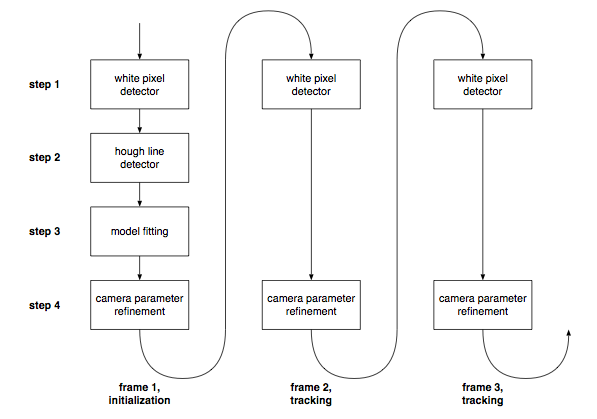
\includegraphics[scale=0.5]{steps.png}
\caption{الگوریتم کلی}
\label{overview}
\end{figure}
برای هر دنباله‌ای از تصاویر مانند شکل \ref{overview} ابتدا در فریم اول، مقداردهی اولیه پارامترهای دوربین (الگوریتم اول) انجام می‌شود که شامل هر چهار قسمت نام برده شده در بالاست. سپس در فریم‌های بعدی الگوریتم دنبال کردن استفاده می‌شود که شامل مرحله‌ی پیدا کردن پیکسل‌های سفید روی خط و بهبود پارامترهای دوربین است.

\subsection{مدل زمین}
فرض شده است که زمین‌های ورزشی، به صورت صفحه هستند. به همین خاطر نگاشت بین مختصات دنیای واقعی و مختصات تصویر یک نگاشت هوموگرافی\LTRfootnote{Homography} است. برای پیدا کردن پارامترهای این ماتریس نیاز به حداقل ۴ نقطه‌ی متناظر داریم. در این مقاله از نقاط تلاقی خطوط زمین به عنوان این نقاط متناظر استفاده شده است.

برای حداقل ۴ نقطه‌ی منتاظر در تصویر و در مدل زمین، باید ۲ خط عمودی در مدل زمین و ۲ خط افقی را در آن بیابیم و منتاظر این خطوط را نیز در زمین پیدا کنیم. حاصل این ۲ خط عمودی و ۲ خط افقی، ۴ نقطه‌ی تلاقی خواهد بود که مختصاتشان را در تصویر و در دنیای واقعی داریم.
\section{مقدار دهی اولیه‌ی پارامترها}
از این قسمت به بعد فرض می‌کنیم که تصاویر در فضای رنگی \lr{YCbCr} قرار دارند و فقط کانال رنگی \lr{Y} که با \textit{\lr{g(x,y)}} نمایش داده می‌شود، در نظر گرفته شده است.
\subsection{تشخیص پیکسل‌های سفید روی خطوط مدل زمین ورزشی}
می‌دانیم که خطوط مدل زمین ورزشی سفید رنگ هستند. ولی پیکسل‌های دیگری هم وجود دارند که سفید رنگ هستند. برای همین منظور به غیر از سفید بودن پیکسل دو شرط تیره‌تر بودن همسایگی و شرط بافت\LTRfootnote{Texture} را نیز در نظر می‌گیریم تا خروجی این قسمت به قدر کافی برای بخش پیدا کردن خطوط مستقیم مناسب باشد.

فرض می‌کنیم که خطوط مدل از $\tau$ پیکسل پهن‌تر نیستند. (\textit{\lr{$\tau$ = 8}}) حال بررسی می‌کنیم که آیا در فاصله‌ی $\tau$ پیکسل از ۴ طرف، مقادر پیکسل‌ها تیره‌تر هست یا خیر. \textit{\lr{l(x,y) = 1}} به این معناست که این پیکسل به عنوان سفید و بر روی خط مدل زمین تشخیص داده شده است.
\begin{figure}
\centering
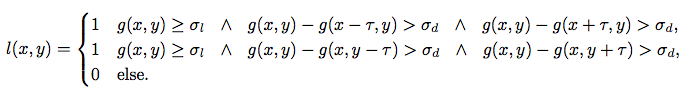
\includegraphics[scale=0.6]{wpixle.png}
\label{wpixle}
\end{figure}
\\

به غیر از شرط بالا، شرط عدم وجود بافت را هم بررسی می‌کنیم. برای اطلاعات بیش‌تر به مقاله مراجعه نمایید.
\subsection{تشخیص خطوط کاندید برای مدل زمین}
\subsubsection{استخراج خطوط مستقیم}
برای این مرحله از تبدیل معروف هاف استفاده شده است. پس از اینکه تبدیل برای یک تصویر حساب شد، در فضای پارامتریک حاصل، نقاط ماکزیمم محلی را که از $\sigma_h \cdot W \cdot H$ مقدار بیش‌تری دارد، نشان دهنده‌ی خطوط هستند. ($W$ عرض و $H$ طول تصویر ورودی است.)

البته این نوع تبدیل گرفتن مشکلاتی از جمله، حاصل شدن تعدادی خط برای خطوط ضخیم در عکس را دارد. این مشکلات توسط مرحله‌ی پردازشی بعدی برطرف شده است.
\subsubsection{بهبود پارامترهای خطوط کاندید}
\begin{figure}
\centering
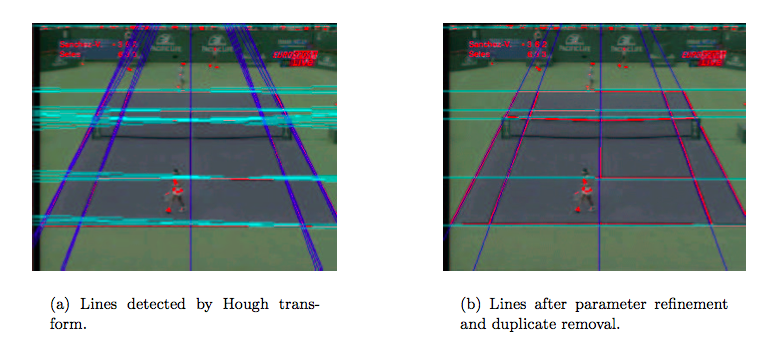
\includegraphics[scale=0.5]{refined.png}
\caption{تأثیر بهبود پارامترهای خط و حذف خطوط تکراری}
\label{refined}
\end{figure}
بهبود پارامترهای خطوط تشخیص داده شده، توسط کم کردن فاصله از پیکسل‌های سفید تشخیص داده شده در مرحله‌ی اول، که نزدیک به این خط هستند انجام می‌شود.

برای این کار از یک \lr{LTS estimator} \cite{LTS} استفاده می‌شود و پیکسل‌های سفید تشخیص داده شده در مرحله‌ی اول که فاصله‌ی آن‌ها از خط در دست بررسی کمتر از $\sigma_r$ (برای مثال ۶ پیکسل) باشد، در این تقریب‌زن مورد استفاده قرار می‌گیرد.

در گام بعدی خطوط تکراری که فاصله‌ی آن‌ها از هم کم باشد و همچنین زاویه‌ی آن‌ها نسبت به هم کم باشد، حذف می‌شوند.

مراحل بهبود پارامتر و حذف خط تکراری آن‌قدر تکرار می‌شود که تعدا خطوط ثابت باقی بماند. برای اینکه تأثیر این مرحله را به خوبی مشاهده نمایید به شکل \ref{refined} توجه نمایید.
\subsection{برازش مدل زمین ورزشی بر خطوط کاندید}
\subsubsection{پیدا کردن تناظر بین خطوط مدل زمین و خطوط کاندید تشخیص داده شده در تصویر}
این مرحله شامل یک جستجوی ترکیبی است که محاسبات سنگینی را می‌طلبد. پس از اینکه تناظر بین خطوط مشخص شد، ما می‌توانیم تناظر بین نقاط را پیدا کرده و ماتریس هوموگرافی را محاسبه کنیم.

برای هرچه سریع‌تر شدن این مرحله ابتدا خطوط را به دو دسته‌ی عمودی و افقی تقسیم می‌نماییم. (عمودی و افقی در مدل زمین معنا دارد) سپس بر اساس فاصله از چپ یا بالای تصویر، خطوط را مرتب می‌کنیم. این مسئله باعث از بین رفتن تناظرهای یکسان که به خاطر خطوط مدل که قرینه هستند ایجاد شده، می‌شود و فضای جستجو را کاهش می‌دهد و باعث افزایش سرعت می‌شود.

حال باید از بین تناظرهای مختلف، آن که مناسب‌تر است را انتخاب کنیم. از آنجایی که اندازه‌گیری میزان خوب بودن یک تناظر کار زمان‌بری است، یک مرحله رد کردن تناظر را معرفی می‌کنیم.
\subsubsection{رد کردن سریع تناظرهای غیر منطقی}
از آنجایی که مدل زمین نمی‌تواند به صورت غیر مساوی در راستای عمودی و افقی مقیاس بپذیرد، برخی از تناظرها را می‌توان سریع رد کرد.

برای ملاحظه‌ی جزئیات به مقاله مراجعه شود.
\subsubsection{محاسبه‌ی امتیاز یک هوموگرافی}
پس از محاسبه‌ی ماتریس هوموگرافی توسط یک تناظر که خروجی مراحل قبل است، می‌توان مدل زمین را (شامل تمام خطوط آن) با استفاده از ماتریس هومگرافی بر روی مختصات تصویر رسم کرد. سپس توسط فرمول شکل \ref{score} امتیاز محاسبه می‌شود.

\begin{figure}
\centering
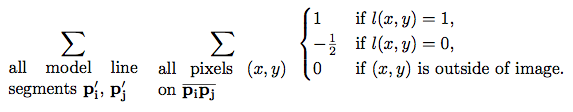
\includegraphics[scale=0.5]{score.png}
\caption{نحوه‌ی محاسبه‌ی امتیاز برای یک خط}
\label{score}
\end{figure}

در پایان آن پارامترهایی (یا ماتریس هوموگرافی) که بیش‌ترین امتیاز را کسب کرده‌اند انتخاب می‌شوند.
\section{دنبال کردن}
فرض می‌کنیم که شتاب حرکت دوربین خیلی کم یا صفر باشد. بر این اساس ابتدا حدسی در مورد پارامترهای دوربین در لحظه‌ی بعد خواهیم زد. سپس توسط تصویر لحظه‌ی بعد که حال نقاط سفید روی خط آن را استخراج کرده‌ایم، می‌توانیم پارامترهای حدس زده شده را بهبود ببخشیم.
\subsection{حدس زدن پارامترهای دوربین}
فرض کنید که $H_t$ پارامترهای دوربین در لحظه‌ی $t$ باشد. اگر پارامترهای دوربین را در لحظه‌های $t$ و \lr{$t - 1$} بدانیم، می‌توانیم حدسی در مورد پارامترها در لحظه‌ی $t+1$ بزنیم.
\[
\hat{H}_{t+1} = H_tH_{t-1}^{-1}H_t
\]
\subsection{بهبود پارامترهای حدس‌زده شده}
در این گام و پس از اینکه حدس در مورد پارامترها زده شد، لازم است که پارامترها با تصویر مطابقت داده شوند. پس ابتدا و برای فریم جدید، پیکسل‌های سفید کاندید روی خطوط زمین بودن استخراج می‌شوند. حال معکوس مارتیس هوموگرافی را محاسبه می‌کنیم.
\[
M = \hat{H}_{t+1}^{-1}
\]
توسط این ماتریس می‌توان تمام پیکسل‌های سفید را بر روی مختصات مدل رسم کرد. هدف پیدا کردن مارتیس $M^*$ است که فاصله‌ی اقلیدسی نقاط سفید از خطوط مدل در مختصات مدل کمینه باشد. برای این منظور از روش بهینه‌سازی \lr{Levenberg-Marquardt} استفاده می‌کنیم.
\begin{latin}
\bibliography{court_model_bib}{}
\bibliographystyle{plain}
\end{latin}

\end{document}